\documentclass[a4paper, 12pt]{report}




%======INFORMATIONEN ZUM WERK=====
\def\docTitle{Erzeugung eines 3D-Modells eines Gebäudes anhand des Grundrisses}
\def\docAuthor{Peter Oehme, Johann Bartel}
%======ALLJEMEINE PAKETE===================
\usepackage[a4paper,left=40mm,top=25mm,bottom=20mm, right=30mm]{geometry} % korrekturränder
\usepackage[utf8]{inputenc} % utf 8 encoding
\usepackage{listings} % Code blocks
\usepackage{fancyhdr}
\usepackage{setspace} % Line spacing
\usepackage{color} % FAARBEN
\usepackage{graphicx} 
\usepackage{titlesec} 
\usepackage[ngerman]{babel} % gutes Deutsch
%\usepackage{glossaries} % Abkürzungsverzeichnis
\usepackage{todonotes}

\usepackage{blindtext}

\usepackage{chngcntr}


\usepackage{lastpage} %Liest Seitenanzahl
% =====FORMAT===========================================================================



\doublespacing %Zeilenabstand 1.5



\titleformat{\chapter}{\LARGE}{\thechapter.}{20pt}{\LARGE}

%\renewcommand{\headrulewidth}{0.4pt} % Ändert die 
%\renewcommand{\footrulewidth}{0.4pt}

\pagestyle{fancy}
%\fancyhead[C]{\docAuthor}

\counterwithout{figure}{chapter} %Abbildungen

%==================================HEADER============================================================================
%\usepackage{scrpage2}
%%\pagestyle{scrheadings}
%\clearscrheadings			%seitenstiel löschen
%\clearscrplain				%das gleiche
%\clearscrheadfoot			%das gleiche
%\rehead{\includegraphics[scale = 1.4]{Bilder/HSLogo.pdf}}
%\rohead{\includegraphics[scale = 1.4]{Bilder/HSLogo.pdf}}
%%\setheadwidth[0pt]{textwithmarginpar}		%Text und bilder im header bis an den rechten blattrand
%\lehead{Hochschule Magdeburg\\
%	Fachbereich: Ingenieurswissenschaften und Industriedesign\\
%	Institut für Maschinenbau}
%\lohead{Hochschule Magdeburg\\
%	Fachbereich: Ingenieurswissenschaften und Industriedesign\\
%	Institut für Maschinenbau}
%\setheadsepline{2pt}
%%\cfoot{\pagemark}
%\renewcommand*{\chapterpagestyle}{scrheadings} %chapterstartseite haben auch ungewöhnliche kopfzeile

\pagestyle{fancy}
\fancyhf{}
\rhead{\docAuthor}
\lhead{Besondere Lernleistung}
\rfoot{Seite \thepage{} von \pageref{LastPage}}

%========================CODEDARSTELLUNG=========================
\lstnewenvironment{code}
{
	\lstset{
		language = Java,
		breaklines  =true,
		commentstyle = \color{green},
		frame = single,
		numbers = left,
		columns=fullflexible}
}
{
}
%========================COMMANDS============
\newcommand{\q}[1]{\glqq#1\grqq} % Zitat mit Anführungszeichen
%\newcommand{\todo}[#1]{\newline\huge \color{red}#1 \color{black}\normalsize}

%\newcommand\todo[1]{\refstepcounter{todo}\marginpar{\color{red}{#1}}\addcontentsline{tod}{subsection}{#1~\thetodo}}

%====================SCHRIFTART ARIAL======================
\renewcommand{\rmdefault}{phv} % Arial
\renewcommand{\sfdefault}{phv} % Arialä

%==========ABKÜRZUNGSVERZEICHNIS=====================
%\makeglossaries
%
%\newglossaryentry{abb}{name={Abb.},description={Abbildung}}
%\newglossaryentry{AutoCAD}{name={AutoCAD},description={Ein Konstruktionsprogramm}}
%


\begin{document}
	
	
	\listoftodos
	\begin{center}
	\thispagestyle{empty}
		%	\vspace*{1cm}
			\textbf{Wilhelm-Ostwald-Schule, Gymnasium der Stadt Leipzig}
			
			\Large
			\textbf{Dokumentation zur Besonderen Lernleistung} \break
			
			\large
			\textbf{Im Fachbereich}\\
			Informatik \break
			
			
			\textbf{Thema}\\
			Erzeugung eines 3D-Modells eines Gebäudes\\ anhand des Grundrisses \break
			
			\textbf{Vorgelegt von}\\
			Johann Bartel und Peter Oehme \break
			
			\textbf{Schuljahr}\\
			2016/2017 \break
			
			\textbf{Externe Betreuer}\\
			Herr Prof. Dr. Gerik Scheuermann, Herr Tom Liebmann \break
			Universität Leipzig
			Fakultät für Mathematik und Informatik \break
			
			\textbf{Interner Betreuer}\\
			Herr Rai-Ming Knospe \\
			
			
			\vspace{0.5cm}
			
\end{center}
	%Bibliographie
%========================CHECKED===============================%
\chapter*{Bibliographische Beschreibung}
Bartel, Johann und Oehme, Peter\\\\
\q{\docTitle}\\\\
  \theseitennr\ Seiten, \totalfigures\ Abbildungen
 
  \newpage
 
 %ABSCHTRAKT
\chapter*{Erzeugung eines druckbaren 3D-Modells eines \\ Gebäudes anhand des Grundrisses}
Die Zielstellung dieser BeLL ist es, den Grundriss eines Hauses, der aus einem Konstruktionsprogramm entnommen wurde, in eine druckbare 3D-Datei zu konvertieren.
Diese Umwandlung wird mithilfe eines Programmes mit eingebetteten selbst entworfenen mathematischen Operationen realisiert.\\\\
Aus dem Grundriss, welcher eine 2D-Datenmenge darstellt, werden die digitalen Anweisungen für die 3D-Strukturen Wände, Grundflächen und \mbox{Eckpfeiler} berechnet. 
Diese Anweisungen lassen sich nach der Umwandlung in einem Modellierungsprogramm für den Druckvorgang umwandeln.
Die Berechnungen der Umwandlung laufen so ab, dass an allen Elementen des finalen Modells komplementäre Stecker angebracht werden, die zusammen als ein Stecksystem fungieren. 
Eckpfeiler dienen hierbei als Verbindungsstücke zwischen den Wänden und Bodenplatten, welche somit für die Stabilität des Objektes  sorgen. 
Das Stecksystem ermöglicht ein Zusammensetzen aller Bauteile zu einem stabilen Modell. 
Dadurch entsteht ein Modell, welches aufgrund der genannten Modifikationen transportabel und geeignet für Präsentationen ist.\\\\
Architekten können die 3D-Darstellung der Immobilie  nutzen, um mehr Eindruck über das Objekt zu erlangen und eine mögliche Inneneinrichtung zu planen.\\\\
Johann Bartel und Peter Oehme

	\tableofcontents
	\chapter{Einleitung}
3D-Druck gehört zu den beliebtesten technischen Neuerungen der letzten Jahre.
Nicht nur im privaten Einsatz, sondern auch im professionellen Bereich finden 3D-gedruckte Objekte immer mehr Anwendung.
Die anschauliche Darstellung bestimmter Elemente ermöglicht dabei auch unerfahrenen Nutzern Zugang zu komplexen Objekten. \\

Naheliegend ist es demzufolge, diese Technik zur Visualisierung von Gebäuden zu verwenden.
Auf Basis des Grundrisses, einer einfachen Form der Darstellung eines Gebäudes, sollte es möglich sein, ein Modell zu erstellen.
Dieses soll in kleine Grundeinheiten unterteilt sein, die über ein Stecksystem zusammengesetzt werden können. \\

Die Umsetzung dieses Problems ist das Ziel dieser Arbeit.
Zur Lösung wird ein Programm in Java erstellt, welches die Umwandlung des Grundrisses in ein Modell übernimmt.

%In den letzten Jahren gewannen 3D-Drucker immer mehr Bedeutung, sowohl für wissenschaftliche als auch für wirtschaftliche Zwecke. 
%Sie werden genutzt, um verschiedene Gegenstände oder Bauteile des Eigenbedarfs selbst herzustellen oder nach Belieben anzupassen. 
%Entsprechend naheliegend war es, dass schnell die ersten Modelle nachgebildet wurden, oder man sich an beliebten Steckbausteinsystemen wie LEGO orientierte, um sich eigene Sets zu drucken. \\
%
%Diese Eignung für den Modellentwurf und Modellbau erweckte auch die Idee, ein Modell eines Hauses zu drucken, welches in sich aus strukturierten Bauteilen zusammengesetzt ist und somit auch das Entfernen einzelner dieser Bauteile erlaubt, um einen einfacheren Einblick in das Modell zu erhalten. 
%Kombiniert mit dem Interesse an der Architektur entstand die Überlegung, ob es möglich wäre, anhand eines Grundrisses, welchen man aus einem Konstruktionsprogramm wie beispielsweise AutoCAD in Form einer .dxf-Datei erhalten kann, ein 3D-Modell des Hauses zu erzeugen, welches mithilfe eines Programmes automatisch in die vorgesehenen Bauteile zerlegt wurde, das im Anschluss von einem 3D-Drucker gedruckt werden kann.
%Dem Nutzer wird demnach nur zuteil, den Grundriss einzuspeisen und die ausgegebenen Bauteile korrekt auszudrucken,  was ihm einen aufwendigen Modellierungs- und Zerlegungsprozess erspart. \\
%
%Ein solches Modell soll dann Architekten als Möglichkeit vorliegen, um ihren Kunden vor dem Kauf eines Hauses näheren Einblick in die Immobilie zu gewähren und mit ebenfalls 3D-gedruckten Möbeln bereits im Voraus erste Einrichtungsideen zu überprüfen. 
%Diese Methode würde auf ein ausgeprägtes dreidimensionales Vorstellungsvermögen des Kunden verzichten und als Ergänzung zum vorgelegten Grundriss funktionieren.\\
%
%Die Umsetzung des Programms erfolgt in der Programmiersprache Java.
%Um die Problemstellung zu bewältigen, musste zunächst eine systematisch einzuhaltende Zerteilung des Modells festgelegt werden. 

	\chapter{Wissenschaftliche Grundlagen}
\section{Planare Graphen}
Zur einfacheren Handhabung wird der Grundriss in einen planaren Graphen umgewandelt. 
Ein planarer, auch plättbarer Graph, ist ein Graph, der in einer Ebene mithilfe von Knoten und Kanten dargestellt werden kann, ohne dass sich zwei oder mehr Kanten schneiden (vgl. Quelle \cite{planarGraph}). 
Jede Fläche des Graphen wird dabei durch mindestens drei verschiedene Kanten beschrieben, die den Rand der Fläche darstellen. 
Die Fläche um den Graphen herum, welche unbegrenzt groß ist, wird äußeres Gebiet genannt.
\begin{Bild}{Schema eines planaren Graphen(Abbildung der Verfasser)}
	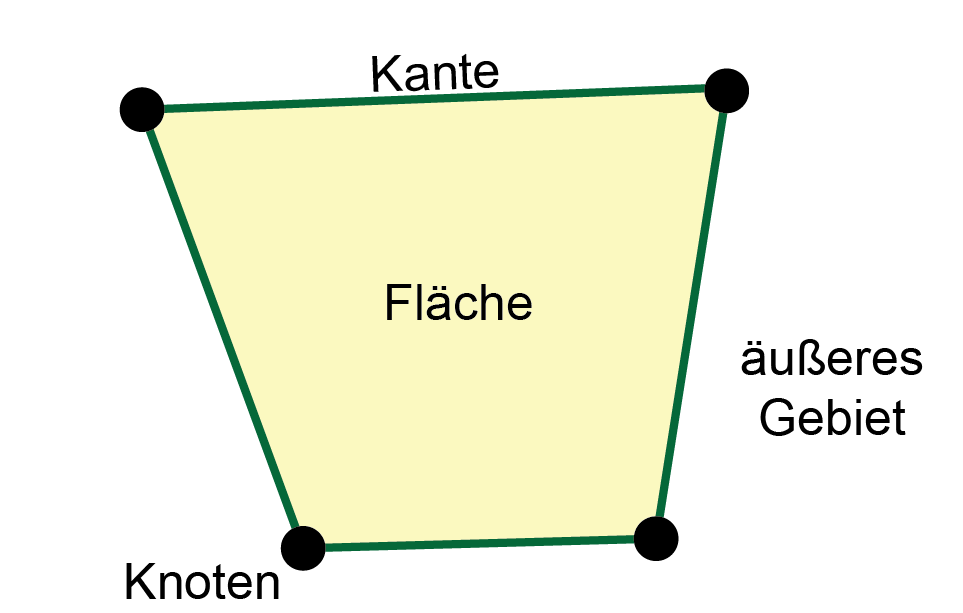
\includegraphics[width = 250px]{Bilder/planarerGraph-11}
\end{Bild}

\section{Doubly connected edge list}
Um planare Graphen ohne Informationsverlust zu speichern wird in der Informatik eine sogenannte \q{Doubly connected edge list} (DCEL) genutzt.
In einer DCEL erhält jede Kante, die aus einem Anfangsknoten und Endknoten besteht, jeweils eine Vorgänger-, Nachfolger-, Zwillingskante und die angrenzende Fläche. 
Durch die Darstellung einer Linie des Grundrisses durch zwei zueinander entgegengesetzt laufenden Kanten wird gewährt, dass sich keine zwei Flächen an einer Kante anliegen.\\
Zudem wird für einen Knoten der DCEL eine ausgehende Kante und für eine Fläche eine anliegende Kante gespeichert (vgl. Quelle \cite{dcel} und \cite{dcelwiki}). \\
Die Kanten der Flächen verlaufen im mathematisch positiven Drehsinn.
Als einzige Ausnahme gilt das äußere Gebiet, welches einen umgekehrten Drehsinn besitzt.

\begin{Bild}{Schema einer DCEL (Abbildung der Verfasser)}
	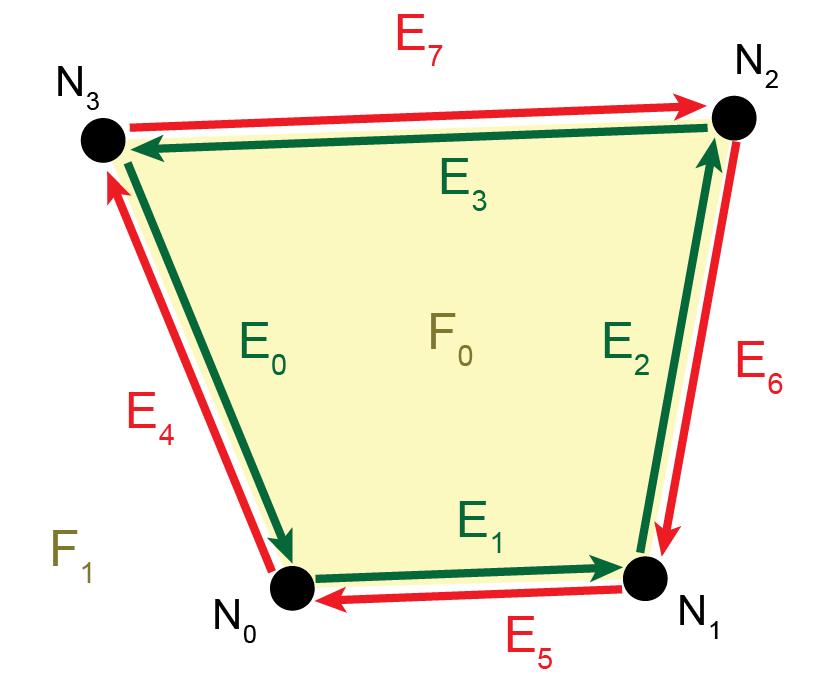
\includegraphics[width=250px]{Bilder/DCEL-10}
\end{Bild}

Folgende Tabellen verdeutlichen die Referenzen der Bestandteilen einer DCEL in Abbildung \thebildnr.\\\\

\begin{tabularx}{\textwidth}{|Y|Y|}
	\hline
	\thead{Knoten} & \thead{ausgehende Kante} \\
	\hline
	$N_0$ & $E_1$ \\
	\hline
	$N_2$ & $E_6$ \\
	\hline
\end{tabularx}\\\\

\begin{tabularx}{\textwidth}{|Y|Y|}
	\hline
	\thead{Fläche} & \thead{anliegende Kante} \\
	\hline
	$F_0$ & $E_3$ \\
	\hline
	$F_1$(äußere Gebiet) & $E_7$ \\
	\hline
\end{tabularx}\\\\

\begin{tabularx}{\textwidth}{|Y|Y|Y|Y|Y|}
	\hline
	\thead{Kante} & \thead{Nachfolger} & \thead{Vorgänger} & \thead{Zwilling} & \thead{Fläche} \\
	\hline
	$E_0$ & $E_1$ & $E_3$& $E_4$& $F_0$ \\
	\hline
	$E_1$ & $E_2$ & $E_0$& $E_5$& $F_0$ \\
	\hline
\end{tabularx}

\section{Oriented Minimum Bounding Box}
Die Oriented Minimum Bounding Box(OMBB) bzw. das orientierte minimale Begrenzungsrechteck einer Fläche ist das Rechteck, welches das komplette Polygon umschließt und dabei den kleinstmöglichen Flächeninhalt besitzt.
Sie wird über den \q{Convex Hull} (konvexe Hülle) eines Polygons berechnet.
Der \q{Convex Hull} ist die kleinste konvexe Menge, in der die Punkte der Fläche enthalten sind.
Mindestens eine Seite des minimalen Begrenzungsrechtecks ist kollinear zu einer Seite der konvexen Hülle.

\begin{Bild}{Beispiel einer konvexen Hülle (vgl. Quelle \cite{ombb})}
	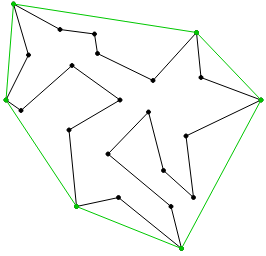
\includegraphics[width = 150px]{Bilder/convex_hull}
\end{Bild}
\begin{Bild}{Eine mögliche Bounding Box (l.) im Vergleich zur OMBB (r.) (vgl. Quelle \cite{ombb})}
	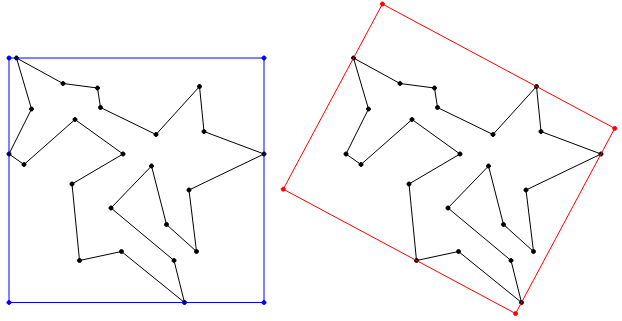
\includegraphics[width = \textwidth]{Bilder/aabb_vs_ombb}
\end{Bild}

\section{AutoCAD}
%Konstruktionsprogramm statt architektenprogramm
AutoCAD ist ein grafischer Zeichnungseditor, welcher zum Erstellen von technischen Zeichnungen und dem Modellieren von Objekten verwendet wird (vgl. Quelle \cite{autocadwiki}).
AutoCAD verwendet dabei einfache Objekte wie Linien, Kreise und Bögen, um auf deren Grundlage kompliziertere Objekte zu bilden.
Zu AutoCAD gehörig wurde das Dateiformat \q{.dxf} entwickelt, welches als Industriestandard zum Austausch von CAD-Dateien dient. \\

\begin{Bild}{Grundriss aus AutoCAD (Screenshot der Verfasser)}
	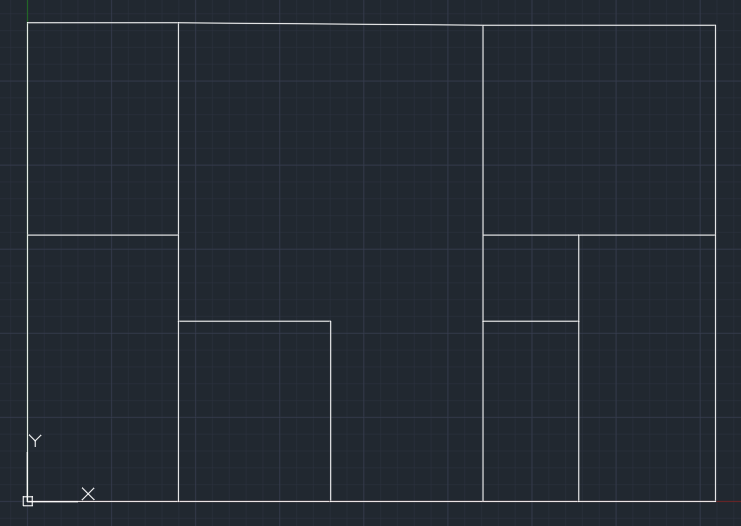
\includegraphics[width=\textwidth]{Bilder/Grundriss}
\end{Bild}

Der Grundriss, welcher als Ausgangspunkt fungiert, wird in AutoCAD erstellt und liegt als .dxf-Datei vor.
Ein Beispiel für einen solchen Grundriss ist in Abbildung~\thebildnr\ zu sehen.

\section{OpenSCAD}
OpenSCAD ist eine kostenlos verfügbare CAD-Modellierungssoftware, welche aus einer textbasierten Beschreibungssprache 3D-Modelle erzeugt (vgl. Quelle \cite{OpenScad}).
OpenSCAD bietet dabei verschiedene Vorteile während des Modellierungsvorganges, beispielsweise das farbige Hervorheben oder die Modularisierung zusammenhängender Objekte. \\

%Modellierung
Die Modellierung von einfachen Basisobjekten in OpenSCAD erfolgt durch das Verwenden von Anweisungen wie \icode{cube()}, \icode{sphere()} oder \icode{cylinder()} und Parametern in Klammern.
Diese Basisobjekte können anschließend durch Mengenoperationen wie Vereinigungen (\icode{union()}), Differenzen (\icode{difference()}) oder Schnittmengen (\icode{intersection()}) und Transformationen wie Skalierungen (\icode{scale()}), Rotationen (\icode{rotate()}) oder Translationen (\icode{translate()}) miteinander verknüpft und kombiniert werden, um neue Objekte nach eigenen Ansprüchen zu erzeugen.

\begin{Bild}{Eine Differenzmenge zwischen einem Würfel und einem Zylinder in OpenSCAD (Screenshot der Verfasser)}
	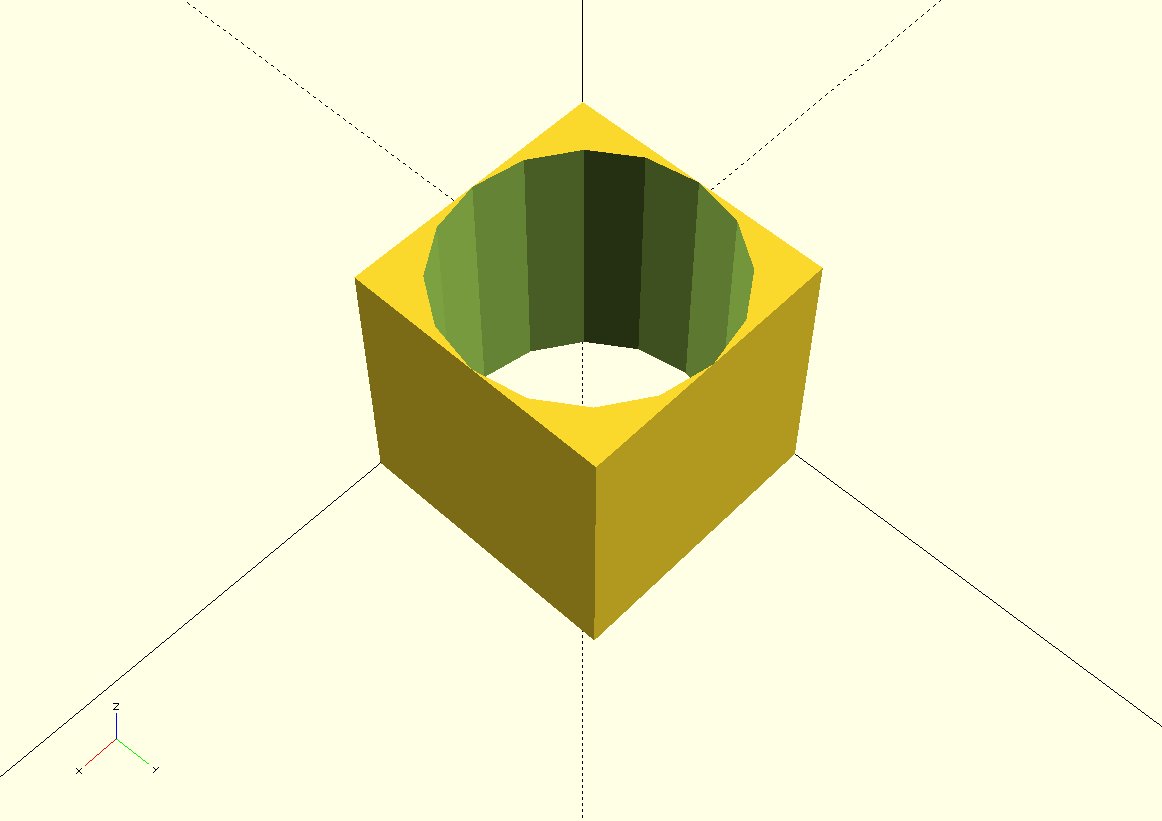
\includegraphics[width= 290px]{Bilder/OpenSCAD_Example}
\end{Bild}

Neben solchen einfachen Objekten wird außerdem die Möglichkeit geboten, komplexere Objekte wie Polygone (\icode{polygon()}) zu erstellen.
Diese können dann ausgehend von einem zweidimensionalen Polygon in Prismen umgewandelt werden (\icode{linear\_extrude()}). \\

Die Anweisungen, welche OpenSCAD zum Modellieren verwendet, werden in einfachen Textdateien im .scad-Format gespeichert.
Die Einfachheit dieser Textdateien erlaubt es, die erhaltenen Anweisungen ohne Umwandlungen in .scad-Dateien zu speichern, welche von OpenSCAD eingelesen, eingesehen und bearbeitet werden können. \\

%Drucken
Die Modelle, die mit OpenSCAD erstellt wurden, können anschließend mit einem 3D-Drucker ausgedruckt werden.
Dazu werden die Modelle in Dateien des .stl-Formats umgewandelt.
Die Konvertierung geschieht entweder über die Benutzeroberfläche von OpenSCAD oder mittels einer Kommandozeilenanweisung.

\section{3D-Drucker MakerBot Replicator\texttrademark\ 2}
%Erklärung 3D-Drucker
Der vorliegende 3D-Drucker ist vom Modell Replicator\texttrademark\ 2 der Firma MakerBot.
Dieser Drucker verfügt über eine höhenverstellbare Grundfläche, auf der das Filament\footnote{Filament bezeichnet das Material, welches der 3D-Drucker zum Drucken verwendet.} aufgetragen und das finale Objekt gedruckt wird.
Ein sogenannter \q{Extruder} erhitzt dazu das zu druckende Filament und trägt dieses auf die Grundplatte auf. 
Mithilfe dieser zwei Hauptbestandteile wird schichtweise Filament aufgetragen, welches aushärtet und so das Objekt bildet. \\
Die Höhe der Grundfläche wird während des Druckvorganges automatisch vom Drucker variiert und nach Abschluss des Drucks wieder auf den Ausgangszustand zurückgesetzt.
Um die Beweglichkeit des Extruders zu garantieren, ist dieser auf drei Achsen befestigt, sodass Motoren ihn auf diesen Achsen verschieben können. \\
Abhängig vom Filament bzw. der Temperatur, bei der dieses aufgetragen wird, der Bewegungsgeschwindigkeit des Extruders und der Filamentstärke, die der Extruder aufträgt, lässt sich die gewünschte Druckqualität anpassen.
Eine niedrige Qualität ist dabei mit einer erheblich kürzeren Druckzeit verbunden. \\
Die Druckzeit wird außerdem von der eingestellten Ausfüllung von geschlossenen Objekten und dem Hinzufügen von Druckhilfen beeinflusst.
So kann man Objekte beispielsweise nicht komplett mit Filament füllen lassen, sondern mit einem Bienenwabenmuster durchsetzen, sodass nur ein geringer Teil des Objektes ausgefüllt, aber dennoch Stabilität gewährleistet wird.
Indem so also ein stark verringerter Betrag an Filament aufgetragen werden muss, wird auch die Druckzeit drastisch reduziert. \\
Zu dem eigentlichen Druckergebnis wird unter jedes gedruckte Element eine dünne Schicht gedruckt, welcher leicht von der Grundplatte und vom gedruckten Modell zu trennen ist und so eine Beschädigung beim Entfernen des Objekts vom Drucker verhindert.
Außerdem werden bei Überhängen zusätzliche Stützen gedruckt, um ein Absacken des noch nicht ausgehärteten Filaments zu verhindern.  \\
Beim Drucken von Objekten ist neben Anpassungen zur Kontrolle der Druckqualität und Druckzeit außerdem zu beachten, dass die Grundfläche eine begrenzten Fläche besitzt.
Entsprechend dieser vorgegebenen Maße sollten alle Objekte in ihrer Größe angepasst werden.
% [28.5 x 15.3 x 15.5 cm]
	\chapter{Vorgehen zur Problemlösung}
\section{Einlesen des Grundrisses}
\subsection{Funktionsweise der Bibliothek \textit{kabeja}}
Den Beginn der Verarbeitung markiert hierbei die Grundrissdatei, in welcher sämtliche Werte, welche im weiteren Verlauf des Programmes relevant werden, enthalten sind.
Das Einlesen der Daten eines Grundrisses, wie in Abb. 5, erfolgt mit der Java-Bibliothek „kabeja“. 
Diese ermöglicht es, aus .dxf-Dateien alle DXF-Objekte eines bestimmten Typs zu erhalten und deren Werte in einer Liste zu speichern und später zu verarbeiten (vgl. Internetquelle 7).
\begin{code}
	public static ArrayList<Line> getAutocadFile
	(String filePath) throws ParseException {
			ArrayList<Line> vcs = new ArrayList<>();
		
			Parser parser =
				ParserBuilder.createDefaultParser();
			parser.parse(filePath,
		8	 		DXFParser.DEFAULT_ENCODING);
		9		DXFDocument doc = parser.getDocument();
		10	
		11		List lst = doc.getDXFLayer("0").
		12	 	 	getDXFEntities(
		13	 		DXFConstants.ENTITY_TYPE_LINE); 
		14		for (
		15	 	int index = 0; index < lst.size(); index++) {
			16			DXFLine dxfline =
			17	 		(DXFLine) lst.get(index);
			18	
			19	 		Line v = new Line(
			20			new Vector(
			21	 		round2(dxfline.getStartPoint().getX()), 
			22	 		round2(dxfline.getStartPoint().getY())),
			23			new Vector(
			24	 		round2(dxfline.getEndPoint().getX()), 
			25	 		round2(dxfline.getEndPoint().getY())));
			26			vcs.add(v);
			27		}
		28		return vcs;
		29	}

\end{code}

\begin{figure}
	\centering
	\includegraphics{example-image-a}
	\caption{Your figure}
%	\label{fig:a}
\end{figure}


In dieser Anwendung wird eine Funktion der Klasse „DXFReader“ verwendet, welche den Pfad zur .dxf-Datei als Parameter übergeben bekommt. 
Aus dieser Datei werden dann alle DXF-Objekte, die mit dem Typen „DXFLine“ übereinstimmen, in einer Liste zurückgegeben. 
Die Koordinaten der Start- und Endpunkte der DXFLines  in dieser Liste werden anschließend in eine Liste von Lines übertragen, welche im weiteren Programmablauf unter anderem für die Umwandlung des Graphen in die DCEL verwendet werden.
\subsection{Funktionsweise der GUI}
\todo{asdf}

\section{Erstellen der DCEL}
\subsection{Line-to-Edge Konvertierung}
In der Hauptklasse des Programms wird nun aus der Liste von Lines ein Graph erstellt. 
Zuerst werden dafür die Lines in Edges einer DCEL umgewandelt und in einer Liste dynamischer Länge gespeichert. 
Die dynamische Länge dieser Liste ist hierbei wichtig, da die Anzahl der Edges im Nachhinein variiert wird.
\begin{code}
	1	private void processData(ArrayList<Line> ls) {
		2		for (Line l : ls) {
			3			edges.add(
			4	 		new Edge(createNode(l.getP1()), 
			5	 		createNode(l.getP2())));
			6		}
		7	}

\end{code}
Die Edges werden während dieses Vorgangs aus je zwei Nodes erstellt, welche später zum Referenzieren der Edges verwendet werden.
\subsection{Twin-Edge Generierung}
Um aus diesen Edges die invertierten Gegenstücke, auch als Zwilingsedges bezeichnet, zu erhalten, werden alle Edges, die in der Liste bereits vorhanden sind, betrachtet und neue Edges hinzugefügt, deren erste Node je der zweiten Node ihrer Zwillingskante entspricht.
Hier ist zu beachten, dass man nicht nach jedem Hinzufügen einer neuen Edge von neuem die Länge der Liste von Edges betrachtet, da man so in eine endlose Schleife gerät. 
Um diesen Umstand zu vermeiden wird also zu Beginn der Verarbeitung die ursprüngliche Länge der Liste festgehalten und nur für diese Einträge ein Hinzufügen von Zwillingsedges durchgeführt.
Direkt nach dem Hinzufügen der neuen Edge wird zusätzlich noch eine Referenz erstellt, die in beiden Edges auf den jeweils zugehörigen Zwilling verweist. 
Diese Referenz dient im folgenden Prozess zur Ermittlung der Winkel zwischen den Edges, welche anschließend verwendet werden, um jeder Edge einen Vorgänger und einen Nachfolger zuzuweisen.
\begin{code}
	1	private void processData(ArrayList<Line> ls) {
		2		for (Line l : ls) {
			3			edges.add(
			4	 		new Edge(createNode(l.getP1()), 
			5	 		createNode(l.getP2())));
			6		}
		7	}
	
\end{code}
Die Edges werden während dieses Vorgangs aus je zwei Nodes erstellt, welche später zum Referenzieren der Edges verwendet werden. 
\subsection{Nachfolger- und Vorgängerermittlung}
\subsubsection{Winkelberechnung an den Knoten}
\subsubsection{Setzen der Referenzen}

\subsection{Flächenerstellung}

\subsection{Vervollständigung der Knoten}

\section{Aufbau der Einzelbauteile}
\subsection{OpenSCAD Java Interface}
\subsection{Corner}
\subsection{Wall}
\subsection{BasePlate}

\section{Druck}
\subsection{\todo{asdf}}


	\chapter{Ausblick}
Die Anwendung ermöglicht eine vollautomatische Umwandlung eines Grundrisses in einzelne Bauteile, aus denen das Modell zusammen gesetzt werden kann.
Entsprechend der ursprünglichen Aufgabe sind damit alle Kriterien erfüllt.
Das Drucken der ausgegebenen Dateien liegt jedoch beim Nutzer, da dies noch nicht vollautomatisch geschehen kann. \\

Als Erweiterungsmöglichkeiten der Anwendung sticht besonders die Aufteilung der Bauteile hervor.
Falls Elemente zu groß für die Grundfläche des 3D-Druckers sind, ist eine Teilung notwendig, damit der Grundriss gedruckt werden kann. \\

Die Möglichkeit, den Nutzer die gewünschten Werte eingeben zu lassen, sowie eine Überarbeitung der Benutzeroberfläche sind weitere mögliche Ansatzpunkte. \\

Den Hauptteil der Laufzeit nimmt zudem die Umwandlung der .scad-Dateien in das .stl-Format in Anspruch.
Eine Optimierung und weitere Vereinfachung der Konvertierung ist äußerst wünschenswert.

%Im aktuellen Entwicklungsstand ist es nur möglich, alle Bauteile einzeln auszudrucken. 
%Dies erhöht jedoch den Filamentverbrauch des 3D-Druckers um ein Vielfaches, weshalb eine Kombination mehrerer Bauteile für einen Druckvorgang zwecks der Reduktion des verwendeten Filaments für den Druck unterstützende Elemente als sinnvoll anzusehen ist. 
%Dafür bietet sich beispielsweise ein gemeinsamer Druck von Wandteilen oder Eckpfeilern anbieten, da diese Objekte weitestgehend ähnliche Ausmaße besitzen und somit eine recht effektive Kombination möglich ist.
%Außerdem liegen momentan lediglich Bauteile vor, welche nur auf einer Druckplatte fester Größe gedruckt werden können. 
%Sollte das zu druckende Objekt größer als die Druckplatte sein, muss es zum Drucken skaliert werden, was jedoch unbedingt vermieden werden soll, da dadurch die Verhältnisse der Stecker zueinander verändert werden und so ein sachgemäßer Aufbau verhindert wird. 
%Um diesen Umstand zu verhindern, soll es in der weiteren Entwicklung möglich sein, überdimensionierte Bauteile weiter in kleinere Untereinheiten zu teilen und so eine Wahrung des Maßstabs zu garantieren. 
%Hierfür muss jedoch ein weiteres Stecksystem, sowie weitere Logik zur Umsetzung und Umwandlung der alten Bauteile konzipiert und implementiert werden.
%Als ferne Zukunftskonzeption, die an den Rahmen der Besonderen Lernleistung anschließt, lässt sich die Umsetzung von 3D-Modellen festmachen. 
%Hierzu zählen kompliziertere Wände mit Schrägen, Fenstern oder Verstrebungen und Dachgestelle, welche als Abschluss auf dem Modell angebracht werden können. 
%Die Komplexität der Aufgabenstellung wird dadurch aber um ein Vielfaches gesteigert, weshalb diese Problematik kein Bestandteil der Besonderen Lernleistung sein wird.
	%\chapter{Quellenverzeichnis}
\begin{thebibliography}{9}
	\bibitem{trapezformel}
			\verb|de.wikipedia.org/wiki/Gau%C3%9Fsche_Trapezformel| (Stand: 21.03.2017, 12:00 Uhr)
		
	\bibitem{dcel}
		 \verb|cs.sfu.ca/~binay/813.2011/DCEL.pdf| (Stand: 25.04.2017, 12:00 Uhr)

	\bibitem{dcelwiki}
		 \verb|en.wikipedia.org/wiki/Doubly_connected_edge_list| (Stand: 25.04.2017, 12:00 Uhr)
		
	\bibitem{OpenScad}
		 \verb|en.wikibooks.org/wiki/OpenSCAD_User_Manual| (Stand: 25.04.2017, 12:00 Uhr)
		
	\bibitem{javaapi}
		 \verb|docs.oracle.com/javase/8/docs/api/index.html| (Stand: 25.04.2017, 12:00 Uhr)
		
	\bibitem{kabeja}
		 \verb|kabeja.sourceforge.net/| (Stand: 12.10.2017, 10:00 Uhr)
		
	\bibitem{openfile}
		 \verb|http://www.journaldev.com/864/java-open-file| (Stand: 28.05.2017, 17:15)
		 
	\bibitem{autocadwiki}
		 \verb|https://en.wikipedia.org/wiki/AutoCAD| (Stand: 05.06.2016, 18:00)
		 
	\bibitem{openscadwiki}
		 \verb|https://en.wikipedia.org/wiki/OpenSCAD| (Stand: 05.06.2017, 18:00)
	
\end{thebibliography}
	
	
%	\printglossary[style=long]
	\listoffigures

\end{document}